\label{chapter:cdft_of_freezing}

The classical density functional theories derived in chapter
\ref{chapter:cdft_intro} were first established to study inhomogenous fluids.
By considering the solid state as an especially extreme case of an
inhomogeneous fluid \cite{HANSEN-CH6}, we can use CDFT to study the process of
solidification. From the perspective of CDFT, solidification occurs once the
density field develops long range periodic structure.  While not expressed in
precisely this language, this approach dates back as far as 1941 with the early
work of Kirkwood and Monroe \cite{KIRKWOOD_MONROE41} and was later
significantly refined by Yussouff and Ramakrishnan \cite{RAMAKRISHNAN79}.

We'll see that the approach of Youssof and Ramakrishnan was very successful at
explaining the solidification in the thermodynamic sense. That is to say, it
elucidates the parameters responsible for solidification but not the dynamical
pathway responsible for the transition. To discuss the pathway toward
equilibrium and the non-equilibrium artifacts introduced along the way into
many solids (e.g. grain boundaries, vacancies, dislocations, etc) we proceed to
extend the CDFT framework using the Dynamic Density Functional Theory (DDFT).
Noting that the full DDFT framework can be intractable in practice, we conclude
by introducing a simplified density functional theory called the Phase Field
Crystal (PFC) theory.

%%%%%%%%%%%%%%%%%%%%%%%%%%%%%%%%
\section{Amplitude Expansions} %
%%%%%%%%%%%%%%%%%%%%%%%%%%%%%%%%

To explore the problem of solidification, we begin with the approximate grand
potential established in equation \ref{cdft_grand_potential} with the external
potential, $\phi(r)$, set to zero,
%
\begin{equation}
    \beta \Delta \Omega[\rho(r)] =
        \int dr \l\lbrace 
            \rho(r)\ln\l(\f{\rho(r)}{\rho_0}\r) - \Delta\rho(r)\r\rbrace
        - \f{1}{2} \Delta\rho(r) \ast C^{(2)}_0(r, r^\prime)
            \ast \Delta\rho(r^\prime).
\end{equation}
%
To make our theory concrete we must choose a suitable reference liquid to set
the parameters $\rho_0$ and $C^{(2)}_0(r, r^\prime)$. We will choose the
reference liquid to be the liquid at the melting point with density $\rho_l$.

Scaling out a factor of $\rho_l$ we can rewrite the grand potential in terms of
a dimensionless reduced density, $n(r) \equiv (\rho(r) - \rho_l)/\rho_l$,
%
\begin{equation}
    \label{gp}
    \f{\beta \Delta \Omega[n(r)]}{\rho_l} =
        \int dr \l\lbrace 
            (1 + n(r))\ln\l(1 + n(r)\r) - n(r)\r\rbrace
        - \f{1}{2} n(r) \ast \rho_l C^{(2)}_0(r, r^\prime) \ast n(r^\prime).
\end{equation}
%
To approximate the density profile in the solid state we can expand the density
in a plane waves,
%
\begin{equation}
    \label{expansion}
    n(r) = \bar{n} + \sum_{\mathbf{G}} \xi_{\mathbf{G}} e^{i \mathbf{G} r}.
\end{equation}
%
Where $\l\lbrace \mathbf{G} \r\rbrace$ is the set of reciprocal lattice vectors
in the crystal lattice and the amplitudes, $\xi_\mathbf{G}$, serve as order
parameters for freezing. $\bar{n}$ is the $k=0$, or equivalently the spatial
average, of the density profile. In the liquid phase all amplitudes are zero
and the average density is uniform, while in the solid phase there are finite
amplitudes that describe the periodic profile of the crystal lattice. As we
have chosen the reference fluid to be the liquid at the melting point with
uniform density $\rho_l$, $\bar{n}$ is zero for the liquid phase at the melting
point (for that reference density) and $\bar{n}$ is the fractional density
change of solidification, defined here as $\eta$, for the solid phase at the
melting point, where
%
\begin{equation}
    \label{eq:eta_def} 
    \eta = \f{\rho_s - \rho_l}{\rho_l},
\end{equation}
%
and in which $\rho_s$ is the macroscopic density of the solid phase.

The amplitudes are constrained by the point group symmetries of the lattice.
Grouping the amplitudes of symmetry-equivalent reciprocal lattice vectors
together we can write the density profile as,
%
\begin{equation}
    \label{amplitudes}
    n(r) = \bar{n}
         + \sum_\alpha \l\lbrace
            \xi_\alpha \sum_{\lbrace\mathbf{G}\rbrace_\alpha}
                e^{i\mathbf{G} \cdot \mathbf{x}}\r\rbrace,
\end{equation}
%
Where $\alpha$ is a label running over sets of symmetry-equivalent reciprocal
lattice vectors. More precisely, if we apply the projection operator of the
totally symmetric representation of the lattice point group to the reciprocal
lattice vectors we may label the distinct linear combinations
\footnote{These linear combinations are all formally equal to zero. It is
important to treat opposite vectors ($\mathbf{v}$ and $-\mathbf{v}$) as
distinct for the sake of calculating the set
$\lbrace\mathbf{G}\rbrace_\alpha$.} with $\alpha$ \cite{KIM99}. The members of
these distinct linear combinations form the set
$\lbrace\mathbf{G}\rbrace_\alpha$.

If we insert equation \ref{amplitudes} into equation \ref{gp} and integrate
over the unit cell of the particular crystal we wish to develop the theory for,
we find,
%
\begin{align}
    \label{amplitude_gp} 
    \f{\beta \Delta\Omega_{cell}}{\rho_l} &=  \int_{cell} 
        dr \l\lbrace (n(r) + 1)\ln\l(n(r) + 1\r) - n(r) \r\rbrace \nonumber \\
    &- \f{1}{2} \l[\bar{n} ^ 2 \rho_l\tilde{C}^{(2)}_0(0) + \sum_\alpha\rho_l\tilde{C}^{(2)}_0
            (\mathbf{G}_\alpha) \lambda_\alpha\vert\xi_\alpha\vert^2\r],
\end{align}
%
Where $\lambda_\alpha$ is the number of reciprocal lattice vectors in the set
$\alpha$ and $\tilde{C}^{(2)}_0(k)$ is the Fourier transform of the direct
correlation function of the reference fluid. The first term in equation
\ref{amplitude_gp} is convex in all of the amplitudes with a minimum at zero.
It is noteworthy, as we will discuss shortly, that the product $\rho_l
\tilde{C}^{(2)}_0(\mathbf{G}_\alpha)$ is a simple function of the structure
factor, $S(k)$\footnote{This follows from the definition of the structure
factor and the Ornstein-Zernike equation}, namely,
%
\begin{equation}
    \rho_l \tilde{C}_0^2(k) = \f{S(k) - 1}{S(k)}\,\,\,\,\forall \,\,k \ne 0.
\end{equation}
%
It follows that solidification must occur when the product $\rho_l
\tilde{C}^{(2)}_0(\mathbf{G}_\alpha)$ (or equivalently, the reference structure
factor $S_0(\mathbf{G}_\alpha)$) is large enough to stabilize a finite
amplitude by creating a new minimum away from zero.  This phenomena is shown
schematically in figure \ref{fig:amplitude_transition} where the grand
potential is projected on to a particular $\xi_\alpha$ axis and plotted for
different values of the reference structure factor. When the reference
structure factors are less than some set of critical critical structure factors 
(denoted as $S^*(\mathbf{G}_\alpha)$), only zero amplitude solutions are
stable.  When the reference structure factors are critical both the zero and
non-zero amplitude solutions are stable and we find liquid-solid coexistence.
Once the reference structure factors are greater than critical one the periodic
crystalline solutions is stable.
%
\begin{figure}
    \centering
    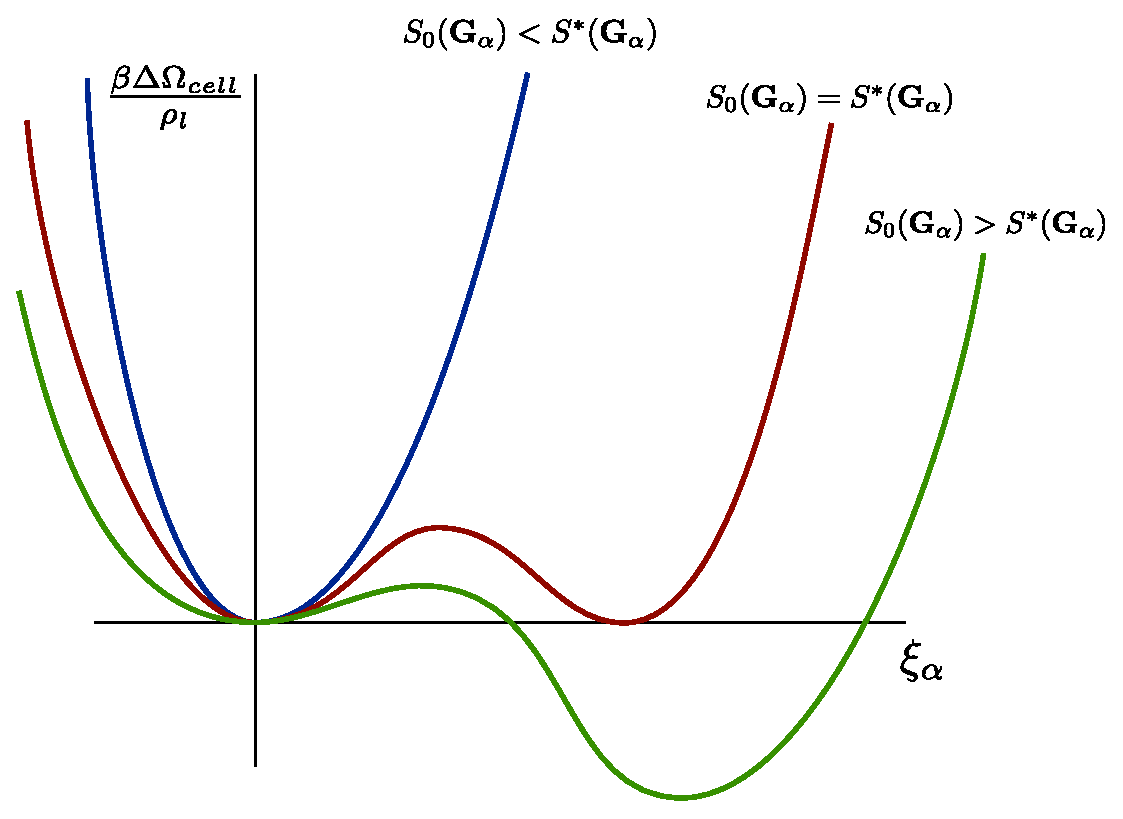
\includegraphics[scale=0.6]{amplitude_transition.eps}
    \caption[Grand Potential through the Solidification transition]{ 
        Schematic view of the grand potential $\beta\Delta\Omega / \rho_l$
        projected on to an $\xi_\alpha$ axis for three different reference
        structure factors. To minimize the grand potential, finite $\xi_\alpha$
        is stable once $S_0(\mathbf{G}_\alpha) > S^*(\mathbf{G}_\alpha)$
    }\label{fig:amplitude_transition}
\end{figure}
%
Furthermore, equation \ref{amplitude_gp} suggests that the set of critical
structure factors, $\lbrace S^*(\mathbf{G}_\alpha)\rbrace_\alpha$ are material
\textit{independent} as no free parameters remain in the grand potential.  As a
consequence, once we specify the symmetry of the lattice a liquid will solidify
into (eg. face-centred-cubic), all materials that undergo this transition
should share these parameters at the melting point. 

Early numerical evidence of this result was supplied by the Hansen-Verlet
criterion \cite{HANSEN69} which states that for a Lennard-Jones fluid the peak
of the structure factor is constant along the melting curve with a value
$\approx 2.85$. It has been noted that in comparing experimental evidence of a
variety of liquids solidifying to fcc structure, most have a peak value close
to 2.8 whereas those solidifying into bcc structures have a peak value around
3.0 \cite{RAMAKRISHNAN79}.

At this level, the CDFT theory of solidification is an infinite order
parameter theory of solidification. We can simplify the theory by truncating
the number of amplitudes we keep in our expansion of the density. This is
justified by noting that only terms from the first few reciprocal lattice families contain the
majority of the grand potential energy of solidification\cite{RAMAKRISHNAN79}.

\begin{table}[H]
    \begin{subtable}{0.4\linewidth}
        \centering
        \begin{tabular}{l c c c}
            \hline 
            Theory & $\tilde{C}(\mathbf{G}_{[111]})$ & $\tilde{C}(\mathbf{G}_{[311]})$ & $\eta$ \\ 
            \hline
            I & 0.95 & 0.0 & 0.074 \\
            II & 0.65 & 0.23 & 0.270 \\
            III & 0.65 & 0.23 & 0.166 \\
            Experiment & 0.65 & 0.23 & 0.148\\
            \hline
        \end{tabular}
        \caption[Freezing parameters for Argon]{Freezing parameters for fcc with
            comparison to Argon experimental results.
        }\label{table:ramakrishnan_argon}
    \end{subtable}
    \hspace{0.10\linewidth}
    \begin{subtable}{0.4\linewidth}
        \centering
        \begin{tabular}{l c c c}
            \hline 
            Theory & $\tilde{C}(\mathbf{G}_{[110]})$ & $\tilde{C}(\mathbf{G}_{[211]})$ & $\eta$ \\ 
            \hline
            I           & 0.69 & 0.00 & 0.048 \\
            II          & 0.63 & 0.07 & 0.052 \\
            III         & 0.67 & 0.13 & 0.029 \\
            Experiment  & 0.65 & 0.23 & 0.148\\
            \hline
        \end{tabular}
        \caption[Freezing parameters for Sodium]{Freezing parameters for bcc with 
            comparison to Sodium experimental results.
        }\label{table:ramakrishnan_sodium}
    \end{subtable}
    \caption[Table of Ramakrishnan results]{Freezing parameters for fcc and
        bcc systems and comparison to experiment from \cite{RAMAKRISHNAN79}.
        Theory I uses one order parameter, theory II uses two order parameters
        and theory III uses two order parameters with a higher (third) order
        expansion in the free energy. $\eta$ is the fractional density change
        of solidification from equation \ref{eq:eta_def}
    }
\end{table}

As seen in table \ref{table:ramakrishnan_argon} and table
\ref{table:ramakrishnan_sodium} theoretical results from a single amplitude
theory (theory I in the results) are poor but improve significantly with two
order parameters (theory II) or higher order expansions of the free energy
(theory III).

%%%%%%%%%%%%%%%%%%%%%%%%%%%%%%%%%%%%%%%%%%%%%
\section{Dynamic Density Functional Theory} %
%%%%%%%%%%%%%%%%%%%%%%%%%%%%%%%%%%%%%%%%%%%%%

In spite of its successes, the CDFT theory of solidification cannot be a
general description of solidification as many materials never fully reach
equilibrium. The resulting microstructure affects the mechanical properties of
the solid. In order to improve our theory we need to examine the pathway
systems take to equilibrium so we can understand these microstructural
features. We begin with a brief overview of non-equilibrium statistical
mechanics.

%%%%%%%%%%%%%%%%%%%%%%%%%%%%%%%%%%%%%%%%%%%%%%%%%%%%%%%%%%%%%%%%
\subsection{Overview of Non-equilibrium Statistical Mechanics} %
%%%%%%%%%%%%%%%%%%%%%%%%%%%%%%%%%%%%%%%%%%%%%%%%%%%%%%%%%%%%%%%%

Consider a non-equilibrium probability distribution over phase space, $f(\q,
\p; t)$. As a function over phase space, its equation of motion is a simple
result of classical mechanics,
%
\begin{equation}
    \label{cm} 
    \f{d f}{dt} = \l\lbrace f, \mathcal{H} \r\rbrace + \f{\partial f}{\partial t}.
\end{equation}
%
Where $\l\lbrace \cdot, \cdot \r\rbrace$ denotes the Poisson bracket,
%
\begin{equation}
    \l\lbrace f, g \r\rbrace = \sum_{i = 0}^N \f{\partial f}{\partial q_i}
        \f{\partial g}{\partial p_i} - \f{\partial g}{\partial q_i}
        \f{\partial f}{\partial p_i}.
\end{equation}
%
Of course, the distribution must remain normalized in time and therefore the 
total time derivative must be zero,
%
\begin{equation}
    \int d\q d\p\, f(\q, \p; t) = 1 \rightarrow \f{d f}{dt} = 0.
\end{equation}
%
Accounting for this conservation law in equation \ref{cm}, the resulting
equation of motion is called the \textit{Liouville Equation},
%
\begin{equation}
    \label{liouville} 
    \f{\partial f}{\partial t} = - \l\lbrace f , \mathcal{H} \r\rbrace
\end{equation}
%
Under appropriate conditions the probability distribution, under the action of
the Liouville Equation, will decay to a stable fixed point $f_{eq}(\q, \p)$ we
call equilibrium,
%
\begin{equation}
    \lim_{t \rightarrow \infty} f(\q, \p; t) = f_{eq}(\q, \p)
\end{equation}
%

Using the non-equilibrium probability distribution, we can also discuss
non-equilibrium averages of the density profile and their associated equations
of motion. The non-equilibrium density is written in analogy with equation
\ref{mean_density} by taking of the classical trace of the density operator
over with the non-equilibrium distribution,
%
\begin{equation}
    \rho(x, t) = \mean{\hat{\rho}(x; \q)}_{ne} =
        \trace{\hat{\rho}(x; \q) f(\q, \p, t)}.
\end{equation}
%
Where $\mean{\cdot}_{ne}$ denotes the non-equilibrium average, (i.e., using
$f(\q, \p,t)$). Just as the non-equilibrium probability distribution is driven
to equilibrium by the Liouville Equation, so too is the density profile by its
own equation of motion.

%%%%%%%%%%%%%%%%%%%%%%%%%%%%%%%%%%%%%%%%%%%%%%%%%
\subsection{Equation of Motion for the Density} %
%%%%%%%%%%%%%%%%%%%%%%%%%%%%%%%%%%%%%%%%%%%%%%%%%

A variety of equations of motion for the density field are known.  For
instance, we can consider the Navier-Stokes equations of hydrodynamics as one
such equation of motion. If we restrict ourselves to diffusion limited
circumstances, we may derive a much simpler equation of motion. To achieve
this result we use the projection operator method, and assume that the 
density operator is the only relevant variable. Quoting the result from
\cite{ESPANOL09} we find,
%
\begin{equation}
    \label{eq:mean_eom}
    \f{\partial \rho(r, t)}{\partial t} = 
        \nabla \cdot \l[\integrate{r^\prime} \mathbf{D}(r, r^\prime, t) 
        \cdot \nabla^\prime \f{\d \F[\rho]}{\d \rho(r^\prime, t)}\r],
\end{equation}
%
where $\nabla^\prime$ denotes differentiation with $r^\prime$, and $\mathbf{D}(r, r^\prime, t)$ is the diffusion tensor,
%
\begin{equation}
    \mathbf{D}(r, r^\prime, t) = \int_0^\infty \mathrm{d}\tau^\prime\,
        \trace{f(\q, \p, t)\hat{\mathbf{J}}(r, 0)
        \hat{\mathbf{J}}(r^\prime, \tau^\prime)},
\end{equation}
%
in which $\hat{\mathbf{J}}(r, t)$ is the local density flux,
%
\begin{equation}
    \hat{\mathbf{J}}(r, t) \equiv 
        \sum_i^N \frac{p_i}{m_i} \d(r - q_i).
\end{equation}
%
Theories using equation \ref{eq:mean_eom} and variations thereof are often
called \textit{Dynamic Density Functional Theories} (DDFT) or at times
\textit{Time Dependent Density Functional Theories} (TDDFT) though we will use
the former throughout this work.

The non-equilibrium diffusion tensor presents a significant impediment to
integrating this equation of motion so in practice it is often approximated.
Following \cite{ESPANOL09}, if we assume that the positions evolve more slowly
than the velocities and that the momenta of different particles are
uncorrelated we can dramatically simplify the diffusion tensor,
%
\begin{equation}
    D(r, r^\prime) = D_0\mathbb{1}\rho(r, t)\d(r - r^\prime).
\end{equation}
%
Where $D_0$ is the diffusion coefficient,
%
\begin{equation}
    D_0 = \f{1}{3 m^2} \int_0^\infty \mathrm{d}t 
        \trace{f(\q, \p, t) p_i(0) \cdot p_i(t)}.
\end{equation}
%
Substituting into equation \ref{eq:mean_eom} we find a simplified equation of
motion originally suggested by \cite{MT1999},
%
\begin{equation}
    \label{eq:marconi_eom}
    \f{\partial \rho(r, t)}{\partial t} = 
        \nabla \cdot \l[ D_0 \rho(r, t)
        \nabla \f{\d \F[\rho]}{\d \rho(r, t)}\r].
\end{equation}
%

The equation of motion can also be written as a Langevin equation. In this
variant the equation of motion is for the density \textit{operator},
$\hat{\rho}$, and the noise is assumed to obey a generalized Einstein relation,
%
\begin{gather}
    \label{eq:langevin_eom}
    \f{\partial \hat{\rho}(x, t)}{\partial t} =
        \nabla \cdot \l[
            D_0 \hat{\rho}(x, t) \nabla \l(
            \f{\d \F[\hat{\rho}]}{\d \hat{\rho}}\r)
            \r] + \xi(x, t), \\
    \mean{\xi(x, t)} = 0, \\
    \mean{\xi(x, t)\xi(x^\prime, t^\prime)} = 
        -2 \nabla \cdot \l[ D_0 \rho(x,t) 
            \nabla \d(x - x^\prime) \d(t - t^\prime)\r].
\end{gather}
%
See Appendix \ref{appendix:noise} for more details on generalized Einstein
relations and \cite{AR2004} for a detailed discussion about equations
\ref{eq:marconi_eom} and \ref{eq:langevin_eom}.

At times, the diffusion tensor is assumed to be constant. This is common place
in many Phase Field Crystal theories. In light of equation
\ref{eq:marconi_eom}, this is akin to assuming the density variations are
small.

Unfortunately, if we were to use the approximate free energy functional
established in equation \ref{cdft_free_energy} in the DDFT of equation
\ref{eq:marconi_eom} or \ref{eq:langevin_eom} we would face a major impediment:
the solid state solutions of the density functional theory approach yield
sharply peaked solutions at the position of the atoms in the lattice. While
this is realistic, they are a major challenge for numerical algorithms that aim
to explore long-time microstructure evolution.  The challenges are two-fold.
First, these sharp peaks require a fine mesh to be resolved resulting in
intractably large memory requirement to simulate domains of any non-trivial
scale. Second, linear stability analysis of most algorithms demonstrates that
the time step size is a monotonically increasing function of the grid spacing,
thus only small time steps can be taken on a fine mesh. This further restricts
the time scales of microstructure evolution that can be practicality explored
to times scales comparable to those of molecular dynamics --perhaps somewhat
longer.

One pragmatic solution to this problem is to further approximate the free
energy functional of equation \ref{cdft_free_energy} in such a way as to
produce a theory that retains the essential physics of solidification but
produces a solid state that is more smoothly peaked. As we will see next, the
Phase Field Crystal (PFC) theory, the topic of this thesis, aims to achieve
precisely this balance.

%%%%%%%%%%%%%%%%%%%%%%%%%%%%%%%%%%%%%%
\section{Phase Field Crystal Theory} %
%%%%%%%%%%%%%%%%%%%%%%%%%%%%%%%%%%%%%%

The phase field crystal theory (PFC) presents a solution to the aforementioned
numerical difficulties faced by DDFT methods by approximating the free energy
in such a way as to retain the basic features of the theory using a smoother
solid state description of density . Starting with the approximate free energy
functional of equation \ref{cdft_free_energy} we proceed as previously by
scaling out a factor of the reference density and changing variables to a
dimensionless density $n(r) = (\rho(r) - \rho_l) / \rho_l$,
%
\begin{equation}
    \f{\beta \F[n(r)]}{\rho_l} = 
        \int dr \l\lbrace (n(r) + 1) \ln( n(r) + 1) - (1 - \beta\mu_0)n(r) \r\rbrace
        - \f{1}{2} n(r) \ast \rho_l C^{(2)}_0(r, r^\prime) \ast n(r^\prime).
\end{equation}
%
We then Taylor expand the logarithm about the reference density or equivalently
$n(r) = 0$, to fourth order,
%
\begin{equation}
    \label{pfc_free_energy} 
    \f{\beta \F[n(r)]}{\rho_l} =
        \int dr \l\lbrace \f{n(r)^2}{2} - \f{n(r)^3}{6} + \f{n(r)^4}{12} \r\rbrace
        -\f{1}{2} n(r) \ast \rho_l C^{(2)}_0(r, r^\prime) \ast n(r^\prime).
\end{equation}
%
Where the linear term can be dropped by redefining the density $n(r)$ about its
average. Most phase field crystal theories also use a simplified equation of
motion as well,
%
\begin{equation}
    \label{pfc_eom}
    \f{\partial n(r, t)}{\partial t} = M \nabla^2 \l(\f{\d \F[n(r)]}{\d n(r)}\r).
\end{equation}
%

As alluded to above, these two simplifications formally make the PFC theory
different from CDFT, turning it instead into a type of Ginzburg-Landau type of
field theory, where $n$ represents an order parameter that becomes periodic in
the solid state. As has been shown in the PFC literature, this apparently gross
over-simplification of CDFT manages to correctly reproduce many of the
qualitative physics of solidification, such as nucleation, grain boundary
misorientation energy, elastic response and dislocations in the solid phase,
vacancy diffusion and creep, grain boundary pre-melting, vacancy trapping, and
numerous other effects. By progressively improving the parametrization of PFC
theories, guided by inspection of the underlying forms, PFC will be able to
better quantitatively model the aforementioned processes.

